\documentclass{svproc}
\usepackage{amsmath}
\usepackage{graphicx}
\usepackage{multirow}
\usepackage{natbib}
\usepackage{caption}
\usepackage[table]{xcolor}% http://ctan.org/pkg/xcolor
\begin{document}
\mainmatter              
\title{The SIR Model}


\author{Jackson Curtis}
\institute{Brigham Young University}

\maketitle           

\begin{abstract}
This project explores parameter estimation of the SIR (Susceptible-Infected-Recovered) Markov chain epidemiology model. I derive the likelihood for the special case where only one of the three states is fully observed. I apply the model to a dataset tracking the spread of a disease through an English boarding school. I calculate several quantities of interest to epidemiologists.
\end{abstract}

\section{Introduction}
The Susceptible-Infected-Recovered (SIR) model is used in epidemiology to describe the spread of a disease throughout the population. Each person in the population is expected to transition from susceptible to ill to recovered with the probabilities given in the transition matrix. An assumption of Markov chain models is that the current state is the only determining factor of the probabilities of transitioning to other states. The following represents our model of interest:
\begin{equation}
\mathbf{E}\begin{bmatrix}
    p_{S,t}       \\
    p_{I,t}      \\

    p_{R,t}     
\end{bmatrix}
=
\begin{bmatrix}
a_{11} & 0 & 0 \\
a_{21} & a_{22} & 0 \\
0 & a_{32} & 1
\end{bmatrix}
\begin{bmatrix}
    p_{S,t-1}       \\
    p_{I,t-1}      \\

    p_{R,t-1}     
\end{bmatrix}
\label{e1}
\end{equation}

The left-hand side represents the expected proportion of the population in each of the categories at time period t and is a function of the transition matrix and the probabilities from the time period immediately preceding. The matrix with the $a_{ij}s$ is the transition matrix for the Markov chain. According to Markov chain assumptions, a person has the probability of transitioning from state i to state j in one time period (regardless of how they got to state i) with the probability given in column i, row j of the matrix. For our case we assign 0 probability of jumping from susceptible to recovered, and a probability of 1 for staying recovered once reaching the recovered state. An assumption we will make throughout the paper is that our initial state will consist of one ill person and the rest susceptible, or, in other words, $P_{I,0}=1/n$ and $P_{S, 0} = (n-1)/n$.

Our dataset of interest is count data of infected students in an English boarding school over fourteen consecutive time periods. An interesting feature that will complicate our analysis is that only the population size (743) and the number sick each day are given. We do not know how many recovered students there were or how many never got sick. We will derive our likelihood to account for this unobserved information. 

Being able to determine the parameters of the model is key to making inference about the spread of the disease to different populations. For example, knowing the parameters that governed the spread of the disease in the boarding school would allow us to make predictions if another school was infected. We could answer questions such as how long the disease will last, and how many people will be infected at once. Knowing these answers will be extremely valuable to decision-makers trying to contain the disease.

Because the columns of the transition matrix must sum to one, only two parameters vary without restriction while the other two are fixed. For ease of interpretation, we will model $a_{12}$ as the probability of catching the disease, and $a_{32}$ as the probability of recovering. These are the two parameters we will obtain through maximum likelihood estimation. 

\section{Deriving the Likelihood}
Because our data is a sequence of observations in time, our data points are not independent or identically distributed. Instead we can write the likelihood as:
\begin{equation}
f(x_1, x_2,...,x_n| a_{12}, a_{32}) = f(x_1| a_{12}, a_{32}) f(x_2|x_1, a_{12}, a_{32}) ... f(x_n|x_{n-1}, a_{12}, a_{32})
\end{equation}
where $x_i$ is the number observed infected at time period i. Each observation is dependent only on the observations that proceeded it.

To deal with the fact that only those in the second state are observed and reported, we can calculate the probabilities of the number of individuals in each of the either two states. To do this, define $R_i$ as a random variable representing the number of people in the recovered state at the start of time period i. Then we can model each piece of the likelihood as

\begin{equation}
f(x_i | x_{i-1}, a_{12}, a_{32}) =\sum_{j=0}^n f(x_i | x_{i-1}, a_{12}, a_{32}, R_i=j)\cdot Pr(R_i=j) 
\label{sum}
\end{equation}

Summing over all possible values of $R_i$ gives us the likelihood of $x_i$ independent of $R_i$.

To demonstrate this, consider the first case, $R_1$. In $R_1$, $Pr(R_1=0)=1$ since no one has had any time to recover. On day two, the original infected person could have recovered (with probability $a_{32}$) or not (with probability $a_{22}$), therefore $Pr(R_2=0) = a_{22}$ and $Pr(R_2=1)=a_{32}$. By summing over the non-zero probabilities in $R_i$, we can calculate the full probability of $x_i$ without knowing how many are recovered or infected. While future states get much more complicated, we can continue to calculate $R_i$ as:

\begin{equation}
Pr(R_i = r + h) = \sum_{j=0}^{x_{i-1}} Pr(H_i=j|R_{i-1}=r-j)\cdot Pr(R_{i-1}=r-j)
\end{equation}

Where $H_i$ represents the number of people who recovered on day i, a number that ranges between 0 and the number of people who were sick on time period i-1.

\subsection*{Renormalizing $R_i$}
Computationally, we will compute 
$R_i$ as we calculate $f(x_{i-1})$. In certain scenarios an observation, $x_i$, may invalidate what we knew about the probability distribution of $R_i$. Consider the simple case of a population of ten people and the observed data of (5, 6, 4, 0, 1). Calculating $R_5$ as derived above, we would conclude that $Pr(R_5 =10)\neq 0$. In other words, from the first four observations we would conclude that it is possible that all ten individuals have already recovered. However, $x_5$ invalidates this. To compensate when new information invalidates old  probabilities, we renormalize the densities so that they still sum to one. This is akin to rolling a dice without observing the outcome and assigning 1/6 to each probability. If you obtain information that the roll was not a one, the proper way to update the probabilities on the other five possibilities is to divide by the sum of the remaining probabilities (5/6). I employ a similar strategy when calculating $R_6$ from $R_5$.

\subsection*{Likelihood Given R}
Now that we have a way to track $R_i$, we can focus on the first piece of \eqref{sum}. If we know r, we can write a closed form of the expression as follows:

\begin{multline}
f(x_i|x_{i-1}, a_{12}, a_{32}, r) = \\ \sum_{h=0}^{x_{i-1}}       {{x_{i-1}}\choose{h}} a_{32}^h(1-a_{32})^{x_{i-1}-h}  {{n-x_{i-1}-r}\choose{x_i-(x_{i-1}-h)}}  a_{12}^{x_i-(x_{i-1}-h)} (1-a_{12})^{n - r - x_i-h}I(x)  \end{multline} $$
\text{where } I(x) = \begin{cases} 1 & \text{for } x_{i-1}-h\leq x_i\leq n-r  \\ 0 &\text{otherwise} \end{cases}$$

This equation breaks down into a sum of two binomial densities, one for how many people recover on time period i and one for how many people get ill on time period i. If the number of people who would need to get sick in order to observe $x_i$ exceeds the number of people who have yet to get sick, the contribution to the probability is 0, which is expressed in the indicator function.

\subsection*{Computational Details}
The resulting likelihood is complex. A triple summation is required to evaluate the likelihood--one for the time periods, one for the number of individuals recovered before day i, and one for the number recovered on day i. The partial derivatives required to obtain the maximum likelihood estimators analytically are intractable, so I used the Nelder-Mead optimization algorithm to maximize the log-likelihood. This requires many evaluations of the log-likelihood. To facilitate faster evaluation, the log-likelihood function was coded in C++.

\section{Evaluating Estimator Performance}
After obtaining a method of calculating maximum likelihood estimates, I tested how they perform at estimating data where the true parameters were known. I was particularly interested in the bias and the variance of the estimates produced from the MLE for different sample sizes and observation times. In order to test this I ran a simulation study where I generated the data using a known Markov chain transition matrix and reported the observed infected at each time period. I then used my likelihood function and Nelder-Mead to estimate the parameters. The following tables summarizes my results for different combinations of the parameters, the size of the population, and the number of time periods.

\begin{table}
\centering
\setlength{\tabcolsep}{5pt}

\begin{tabular}{|c|c|c|c|c|c|c|c|}
\hline
Pop. & No obs. & $a_{12}$ & $a_{32}$ & 95\% CI on $\hat{a}_{12}$ & 95\% CI on $\hat{a}_{32}$ & $\hat{a}_{12}$ sd &$\hat{a}_{32}$ sd  \\ \hline 
743 & 14 & 0.0848 & 0.3420 &\cellcolor{green!25}(0.0845, 0.0857) & \cellcolor{green!25}(0.341, 0.345) & 0.0070 & 0.0212 \\ \hline
500 & 14 & 0.02 &0.3 & \cellcolor{red!25} (0.020, 0.021) &\cellcolor{red!25}  (0.305, 0.319) &0.0046 &0.0766 \\ \hline
473 & 14 & 0.0848 & 0.3420 &\cellcolor{green!25} (0.084, 0.086) & \cellcolor{green!25}(0.340, 0.345) &0.0087 & 0.0271\\ \hline
200 & 6 & 0.1 &.3 &\cellcolor{red!25} (0.101, 0.104)&\cellcolor{red!25}  (0.301, 0.314)&0.0174 & 0.0760\\ \hline 
100 & 14 & 0.2 & 0.7 &\cellcolor{red!25} (0.202, 0.206) & \cellcolor{green!25}(0.700, 0.708) & 0.0269 &0.0482 \\ \hline
100 & 14 & 0.7 & 0.2 &\cellcolor{green!25}(0.700, 0.707) & \cellcolor{red!25} (0.222, 0.225) & 0.0435 & 0.0214 \\ \hline
100 & 14 &0.5 &0.5 &\cellcolor{red!25} (0.505, 0.513) &\cellcolor{red!25} (0.534, 0.537)&0.0450 & 0.0405\\ \hline

50 & 20 & 0.1 &0.3 &\cellcolor{green!25}(0.099, 0.104) & \cellcolor{blue!25} (0.282, 0.291) & 0.0270 & 0.0500\\ \hline

20 & 8 & 0.4 & 0.3 & \cellcolor{red!25} (0.405, 0.422) & \cellcolor{red!25} (0.304, 0.315)& 0.0966 & 0.0668\\ \hline



\end{tabular}
\caption{Simulation results for 500 simulations of each scenario. Green means parameter is within interval, red if below interval, blue if above. }
\label{tab1}
\end{table}

The results of the simulation show that our method of estimation approximates the true values quite well. While the truth was not contained in all of the confidence intervals on the predictors, many scenarios produced unbiased estimates, and the bias appears to be small in all cases. It is unclear whether bias comes from the likelihood itself or the Nelder-Mead approximation of the maximum likelihood. In addition, Table \ref{tab1} shows that the standard deviations of the estimate were small and decrease inversely with the size of our population. 

\section{Analysis}
\subsection*{Boarding School Data}
Having shown a reliable way to estimate the parameters, parameters for the boarding school data can be estimated. These estimates will be useful for predicting what would happen if another group was exposed to the same disease. Table \ref{tab2} gives the parameter estimates. According to the estimates, a susceptible individual has about a 1/12 chance of getting sick any given day, and a sick person has a 1/3 chance of recovering on any given day.
\begin{table}
\centering
\setlength{\tabcolsep}{30pt}
\begin{tabular}{l|c|c|}
\cline{2-3}
&\multicolumn{2}{|c|}{Boarding School Parameter Estimates} \\
\cline{2-3}
&$\hat{a}_{12}$ & $\hat{a}_{32}$ \\ \hline
All Data&0.0848 & 0.3420 \\ \hline
Post-Ramp Up&0.3515 & 0.4525 \\ \hline
\end{tabular}
\caption{MLE estimates for all boarding school data, and data subset after four days}
\label{tab2}
\end{table}

A concern to draw attention to however is model fit. The data does not do a particularly good job of meeting model assumptions. One assumption of the model is that once a disease is present, the entire population is completely exposed to it. However, the boarding school data seems to suggest a ramp up time where the probability of getting infected increases as more people carry the infection. The left side of Figure \ref{plot1} demonstrates this lack of fit graphically by simulating 200 situations where the true parameters are our MLEs, plotted against the actual boarding school data. Clearly, the model isn't well accounting for ramp up time in the data.

\begin{figure}
\centering
\begin{minipage}{.4\textwidth}
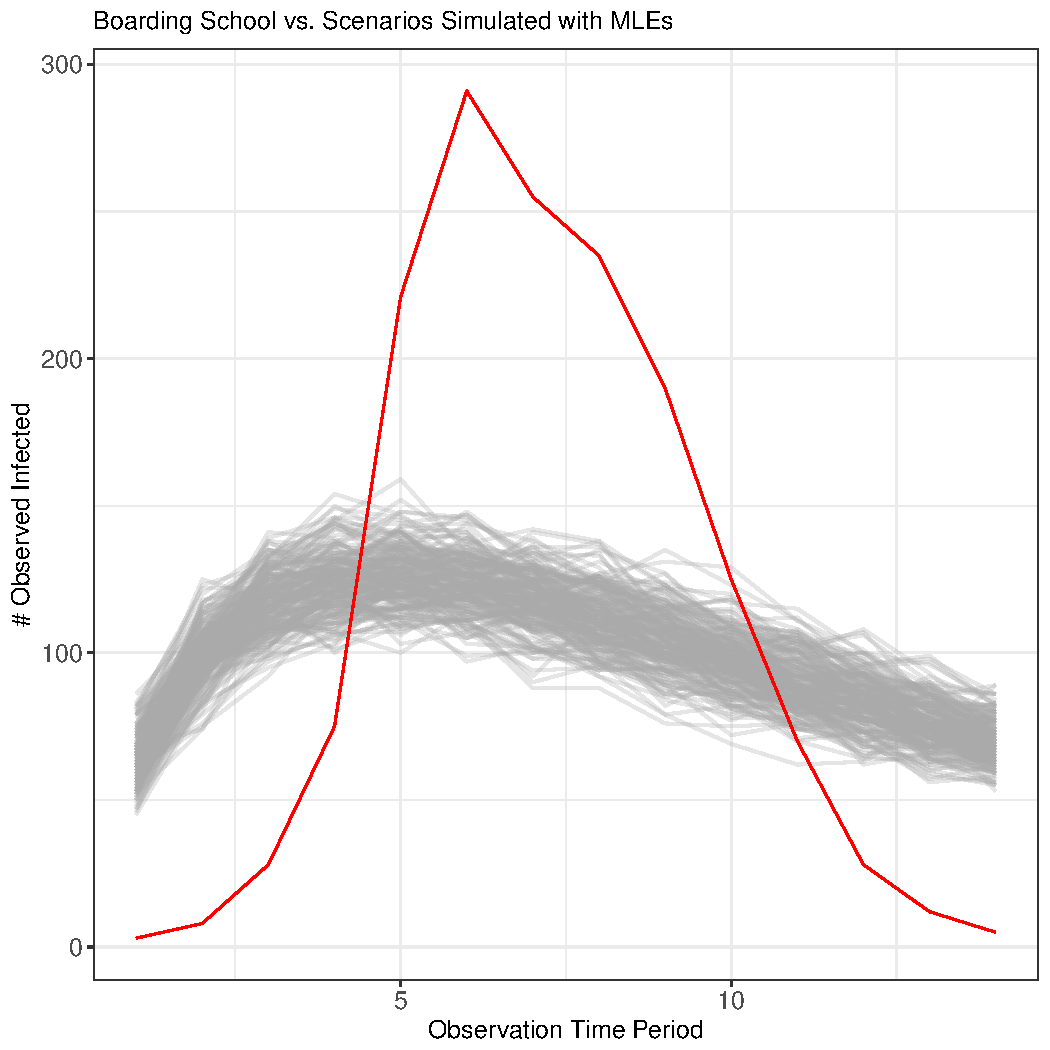
\includegraphics[width=1\linewidth]{LackOfFit.pdf}
\end{minipage}%
\begin{minipage}{.4\textwidth}

\centering
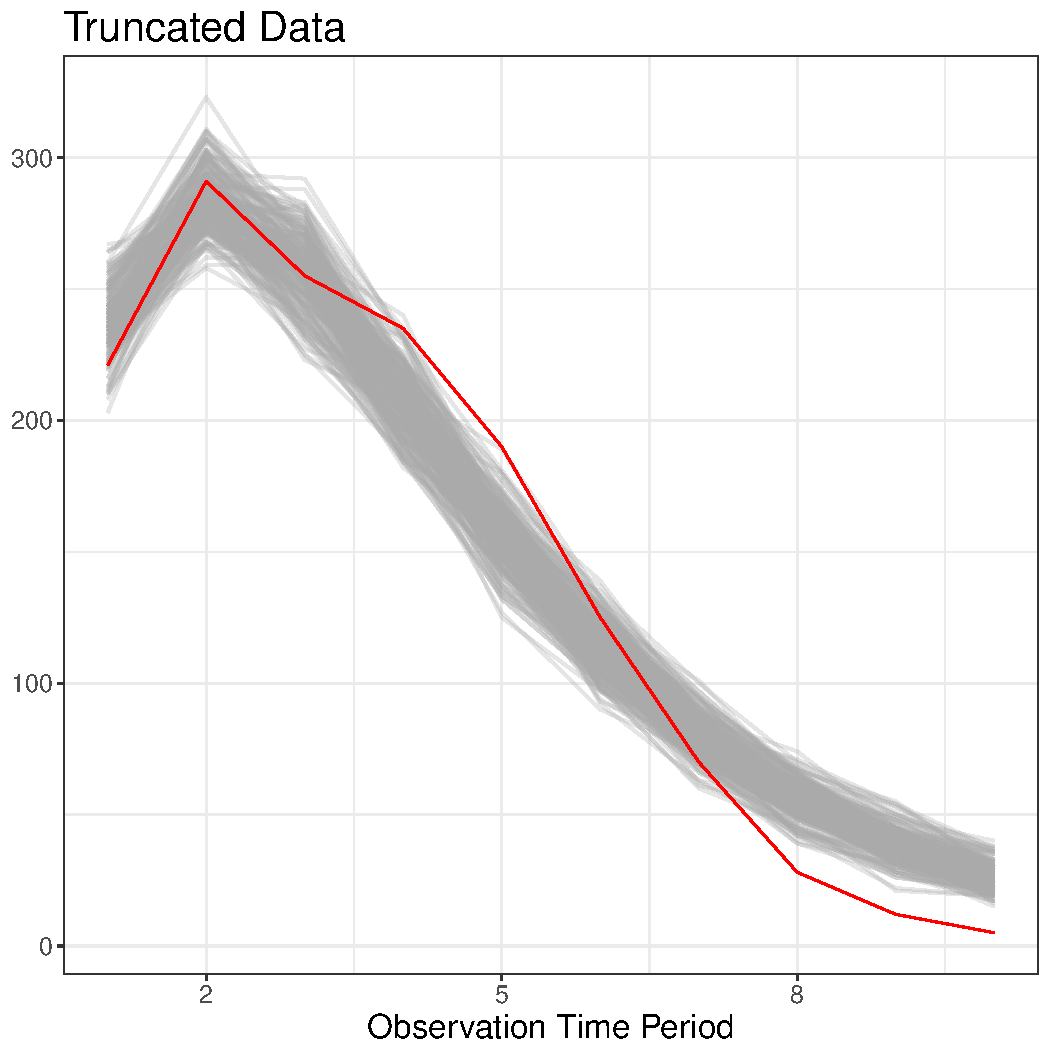
\includegraphics[width=1\linewidth]{BetterFit.pdf}
\end{minipage}
\caption{Actual data vs. 200 simulations using MLE as parameters for full dataset and dataset without first four days}
\label{plot1}
\end{figure}

The model might work better, however for smaller, tight-knit populations where one infection is likely to expose the entire population. For example, instead of an entire school, a classroom might better meet the assumptions of the model. One way to address this issue for more diverse populations is to estimate the parameters based only on the days after the disease has been exposed to the whole population. If we remove the first four data points, and make a rough estimate that 680 students have not yet been infected at that point, we can get data that meets our model assumptions much better, as shown on the right in Figure \ref{plot1}. When choosing whether or not to use the SIR model, epidemiologists should consider the size of the population and the way the population is exposed to the disease.



\subsection*{Inference on Model}

In situations where the model fits the data well, knowing the parameters allows us to make many useful conclusions about the spread of the disease. For example, Equation \eqref{e1} allows us to calculate the expected proportion in any category at any given time. To do this one only needs to obtain estimates for the parameters, and then using the starting conditions, iterate repeatedly until the desired time period is reached. %Possibly add a graphic of this phenomenon 
\begin{figure}
\centering
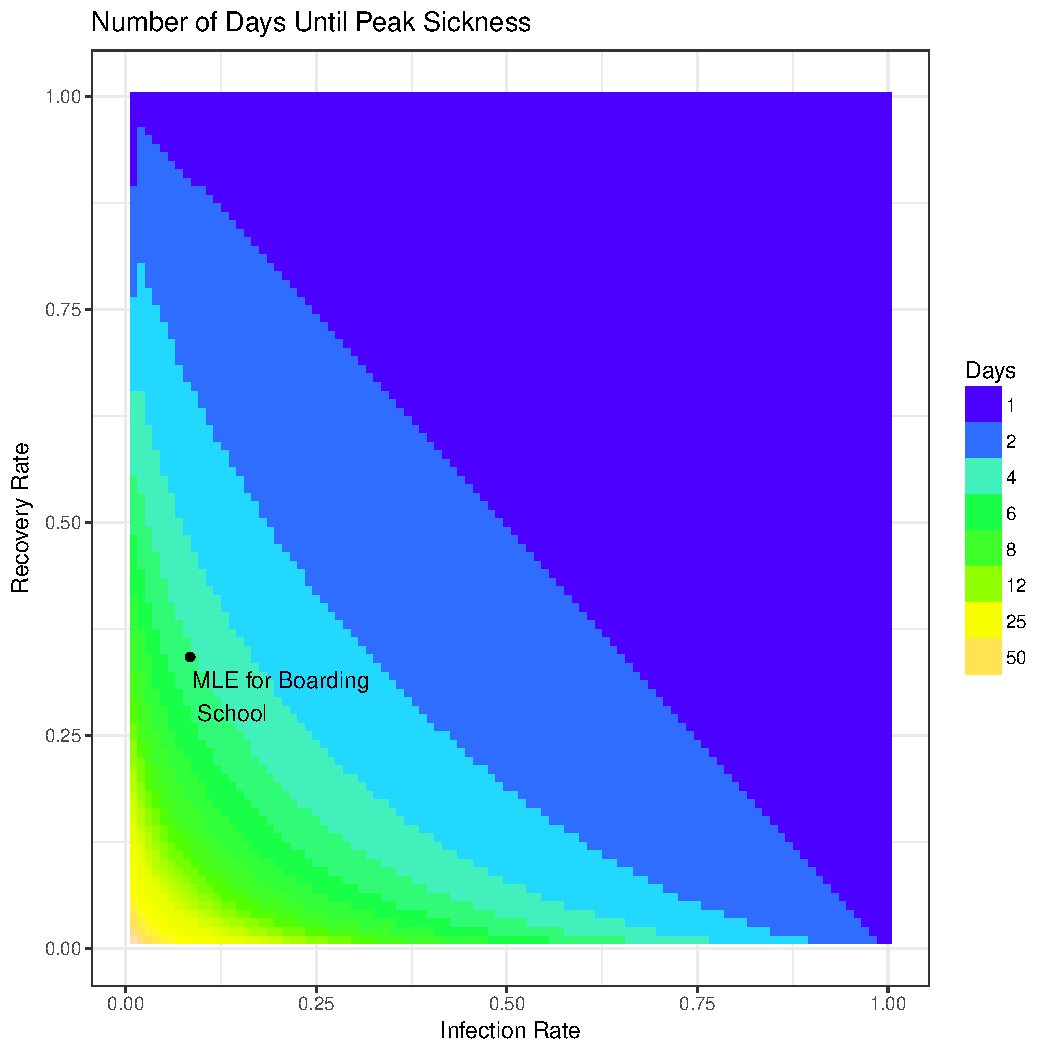
\includegraphics[scale=.7]{DayGrid.pdf}
\caption{A heat map showing when peak illness will be reached for different parameter combinations}
\label{plot2}
\end{figure}

Another useful inference from this model is information about peak illness times. Knowing when the peak will be reached and how many people will be sick could be extremely useful for planning and supplying hospitals. By doing a grid search over different combinations of the parameters, I simulated how long it will take to reach the peak and how many people will be ill when the peak is reached for many possible combinations of the parameters. 


Figure \ref{plot2} shows the number of time periods after initial exposure until the maximum number of people are ill. The number of time periods increases exponentially as the parameters decrease. For any case $a_{12}+a_{23}>1$ the max sickness will be reached the first day because that is when the most people are at risk. 

\begin{figure}
\centering
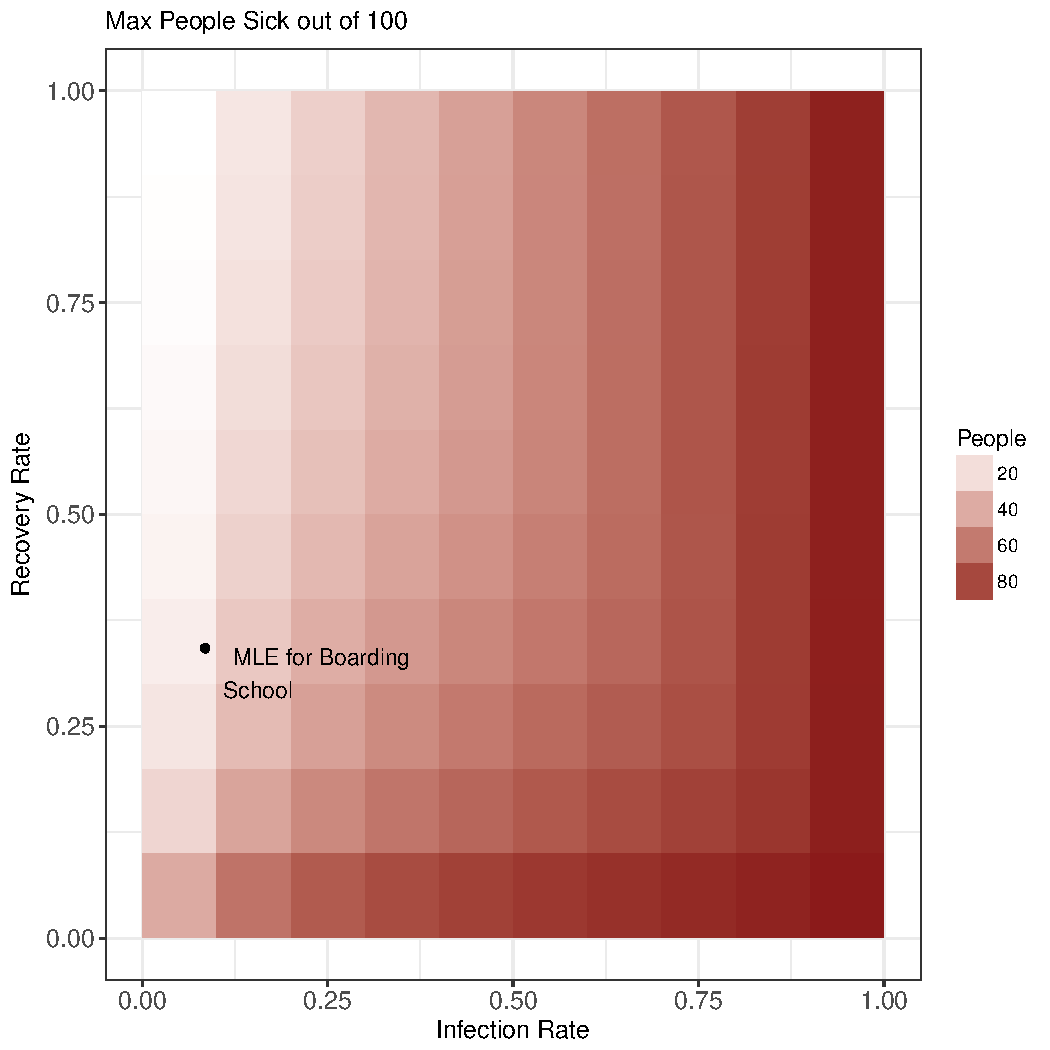
\includegraphics[scale=.7]{MaxGrid.pdf}
\caption{Heat map showing the maximum number of people infected at once}
\label{plot3}
\end{figure}

Figure \ref{plot3} shows the number number of people who will be sick when the peak illness is reached. For the simulation I used a population of 100, but in general any n will remain almost proportional, except for small differences due to the initial assumption of one ill person introducing the disease. In general, a low recovery rate and high infection rate will result in the most people sick at the same time.

Table \ref{tab3} shows reasonable ranges of how many people could be sick at once for several combinations of the parameters for a population size of 100. 
\begin{table}
\centering
\setlength{\tabcolsep}{5pt}
\begin{tabular}{|c|c|c|}

\hline
%\multicolumn{2}{|c|}{Boarding School Parameter Estimates} \\ \hline 
$a_{12}$ & $a_{32}$ & 95\% Quantiles from Simulation \\ \hline
0.0848 & 0.3420 & (15, 27) \\ \hline
0.2 & 0.5 & (22, 35) \\ \hline
0.4 & 0.2 & (51, 69) \\ \hline
0.1 & 0.1 & (34, 50) \\ \hline

\end{tabular}
\caption{The maximum number of ill people (out of 100) fell in these intervals 95\% of the time.}
\label{tab3}
\end{table}

\section{Conclusion}
Epidemiologists use the SIR model to forecast the progression and spread of a disease over time. Having accurate estimators for the parameters of the SIR model is vital to make accurate forecasts. Statisticians can assist in this effort by deriving ways to estimate the parameters using as much information as possible. In this case our only observed data was the number infected at one time. Other cases might present different information such as counts of those sick and recovered but an unknown population size or a situation where the population size is not static. Good estimators will take advantage of all possible information. 

By deriving the maximum likelihood estimators, I have provided tools for epidemiologists to track disease and make predictions. In addition, simulations of data provide an excellent tool for assessing model fit and the appropriateness of the SIR model. Inference on the SIR model benefits from the Markov assumptions. Many quantities of interest (expected values, time spans) are easily calculated from the transition matrix. 

\nocite{*}
\bibliographystyle{spbasic}
\bibliography{refs}

\end{document}

\caption{Simulated data vs. real data using our fifth observation as "Day 1"}
